\section{Verification methods}
\label{verification}

Verification approaches are outlined in figure \ref{fig:verification}. 
(A) represents verification efforts that base their analysis on the low-level code that is or will be deployed on the distributed ledger. Those tools include K/KEVM \cite{Hildenbrandt2017}, Lem (with their possible proofs in Coq or Isabelle/HOL) \cite{Hirai2017}, and F* \cite{Bhargavan2016,Grishchenko2018}.
Tools listed in (B) use the low-level code and decompile it into an IR to reason about properties in the contracts like Securify \cite{Tsankov2017}, Mythril \cite{Mueller2018}, Oyente \cite{Luu2016,Albert2018}, ECF \cite{Grossman2017}, and Maian \cite{Nikolic2018}. ZEUS is an exception as it uses a high-level language to compile an IR and is not verifying properties based on the low-level code \cite{Kalra2018}.
(C) describes tools that reason directly on the high-level code. Solidity can be annotated with Why3 statements to reason about the correctness of the contract \cite{Reitwiessner2015Why3}. Oyente can be used as well, but will compile code into an IR. Those methods can help to find bugs in contracts, but since they do not operate directly on the low-level code, they rely on verified compilers to infer properties like safety, correctness, or liveness.


\begin{figure}
\label{fig:verification}
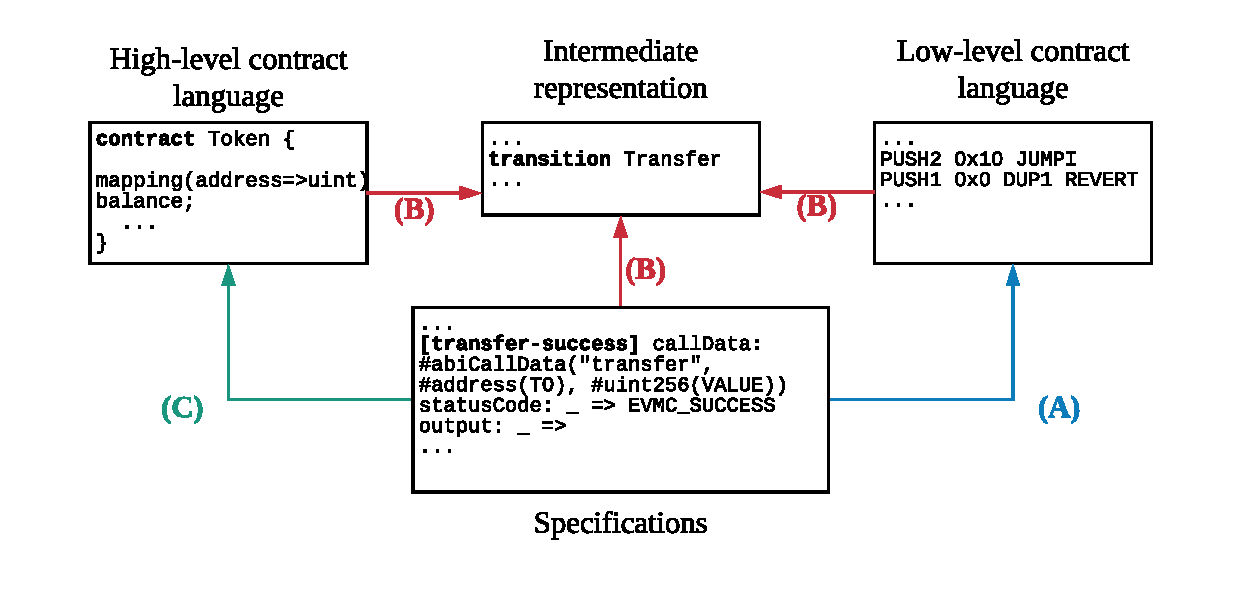
\includegraphics[width=\textwidth]{fig/Verification.pdf}
\caption{Different approaches of verification tools regarding their source for deriving a model or a set of formulas representing the system. Methods listed in (A) directly verify properties from the model or set of formulas from the low-level code. (B) describes tools using an IR from a high-level langauge or from the low-level code to verify the system. Last, (C) describes methods for verifying properties directly from the high-level code.}
\end{figure}

\subsection{Overview}

Verification efforts can be characterised by five criteria \cite[173]{Huth2004}. From these, we adopt three and fixate the other two. 
The application domain concerns smart contracts on a deterministic distributed ledger.
On these ledgers smart contracts are \emph{immutable}, hence, verification before or during, but latest, before deployment, is desirable. Otherwise, they can only be used to find bugs that are already introduced in the software and mostly requires significant efforts to resolve or update the contracts.
Additionally, we included the language that is covered by the specific tool as well as the availability of source code.
This leaves us with the following criteria.
Table \ref{tab:model} presents an overview of the tools we have considered for this survey.

\begin{itemize}
\item \emph{Approach}: In proof-based verification, the system is represented by a set of formulas, while in model-based verification the system is a model. Properties are represented as formulas. The goal is to either proof (proof-based) or to compute whether a model (model-based) satisfies these properties. Proof-based methods typically derive a formal definition of the distributed VM and then try to verify properties of a smart contract. Model-based methods build a model directly from the smart contract and verify the properties with an implicit model of the VM.
\item \emph{Automation}: Fully automated approaches have a set of properties and automatically build a model for the system based on an input (like the source code). Partial automation typically requires defining properties or using a proof-assistant (e.g. Coq or Isabelle/HOL) to define and check proofs.
\item \emph{Coverage}: Property-based verification is concerned with selected parts of the system, while full covers the system as a whole.
\item \emph{Languages}: Lists the languages that are currently, as of September 2018, supported by the methods. Some of the general tools like Lem, F*, K, and Coq can be used for any languages. However, we only list the ones where current research is done.
\item \emph{Source}: Indicates whether the tools and the verification work is available as open source. This criterion is interesting to verify results, experiment with the available tools, and potentially expand them.
\end{itemize}

\begin{table*}
\renewcommand{\arraystretch}{1.3}
\centering
\caption{Overview of model and proof-based verification tools for smart contracts.}
\label{tab:model}
\begin{tabularx}{\textwidth}{XXXXXXr}
\toprule
\textbf{Tool} & \textbf{Approach} & \textbf{Automation} & \textbf{Coverage} & \textbf{Languages} & \textbf{Source} & \textbf{Ref.} \\ \toprule
\emph{Securify} & model & full & full & Solidity, EVM & open & \cite{Tsankov2017} \\
\emph{Mythril} & model & full & property & EVM & open & \cite{Mueller2018} \\
\emph{Oyente} & model & full & property & Solidity, EVM & open & \cite{Luu2016,Albert2018} \\
\emph{ZEUS} & model & full & property & Solidity, Go, Java & closed\textsuperscript{\dag} & \cite{Kalra2018} \\
\emph{ECF} & model & full & property & EVM & open & \cite{Grossman2017} \\
\emph{Maian} & model & full & property & EVM & open & \cite{Nikolic2018} \\ \midrule
\emph{$\mathbb{K}$} & proof & partial & full & EVM, IELE & open & \cite{Hildenbrandt2017,Park2018} \\
\emph{Lem} & proof & partial & full & EVM & open & \cite{Hirai2017,Amani2018} \\
\emph{Coq} & proof & partial & partial\textsuperscript{\ddag} & Scilla, Michelson & open & \cite{Sergey2018,DynamicLedgerSolutions2017} \\
\emph{F*} & proof & partial & partial\textsuperscript{\ddag} & EVM & open & \cite{Bhargavan2016,Grishchenko2018} \\
\bottomrule
\end{tabularx}
\justify
\textsuperscript{\dag} We were not able to find open source code. \\
\textsuperscript{\ddag} Theoretically these tools have a full coverage. However, implementation is as of September 2018 not completed.
\end{table*}




\subsection{Tools}
Model-based methods mostly arise from the need to check contracts for known vulnerabilities. After the DAO and Parity vulnerabilities were known, tools were developed to find similar patterns in other contracts. The proof-based methods arise from the need to proof contracts secure. This requires a formal semantics of the VM and the low-level language. Overall, these methods are used to prevent future vulnerabilities but depend on an exact definition of properties and rigorous formal semantics.

\subsubsection{Model-based}
Securify is a domain-specific model checker for smart contracts \cite{Tsankov2017}. It compiles EVM bytecode to semantics facts and then uses Datalog to define compliance and violation properties to verify the semantic facts. It classifies behaviours of a contract in compliance (matched by compliance properties), violations (matched by violation properties) and warnings (matched by neither). 
Mythril is a symbolic execution of EVM bytecode \cite{Mueller2018}. EVM bytecode is disassembled into a Mythril object, and propositional logic is used to reason about the state space represented as a graph. 
% It is based on the IR LASER \cite{Mueller2018LASER}.
Oyente \cite{Luu2016} and its proposed extension EthIR \cite{Albert2018} build a model from EVM bytecode to verify pre-defined properties. Properties include transaction ordering dependencies, timestamp dependencies, mishandled exceptions, and reentrancy.
ZEUS uses Solidity or Java and Go (as Hyperledger Fabric contracts) as its basis for evaluation \cite{Kalra2018}. It compiles these contracts into an abstract language. Next, properties defined in XACML are used to reason about the contract. The properties together with the abstract language contract get translated to LLVM bitcode for symbolic execution and verification of the properties.
Effectively Callback Free (ECF) objects are a property that is analysed for Ethereum smart contracts\cite{Grossman2017}. A callback method opens up the possibility to change the state of an object (contract) from an external object (contract), which makes reasoning difficult. 
%The authors show that most Ethereum contracts are ECF except for those subject to the vulnerabilities similar to the DAO bug (also referred to reentrancy in other work).
Maian works by symbolic execution of a model of EVM bytecode contracts to find trace vulnerabilities \cite{Nikolic2018}. These vulnerabilities include contracts that leak Ether to unintended parties, can be killed by arbitrary users or lock Ether that cannot be received. 
%They apply their method to verify these properties in real-world contracts.

\subsubsection{Proof-based}
K is a general purpose framework for defining programming languages \cite{Rosu2007}. It is used to build a K representation of the EVM, called KEVM \cite{Hildenbrandt2017}. 
%This VM has been successfully tested against the official test-set of the Ethereum Foundation for any new EVM implementation. 
%Contracts like ERC20 can be specified in K as well \cite{Park2018}. 
A contract can be formally verified using the compiled bytecode, the K contract, and the KEVM virtual machine. Moreover, K is used to defined IELE \cite{Kasampalis2018} and can be used to verify contracts based on this VM.
Lem is used to defining language semantics and can be used to derive implementations in OCaml and enable proof-based verification using Coq, HOL4, or Isabelle/HOL \cite{Mulligan2014}. The EVM has been defined in Lem and subsequently contracts verified using the semantic definition \cite{Hirai2017}. This work is extended by \cite{Amani2018}. 
%The Lem definitions and smart contract verification are pursued by \citeauthor{Hirai2018} at the Ethereum Foundation \cite{Hirai2018}.
Coq is an interactive theorem prover that can be used for any language theoretically. In practice, Scilla is defined in Coq, and there are ongoing efforts to verify Scilla contracts \cite{Sergey2018}. Further, Coq is intended to be used together with the Michelson language \cite{DynamicLedgerSolutions2017}.

\citeauthor{Bhargavan2016} propose to convert Solidity and EVM bytecode to F* \cite{Bhargavan2016}. This can then be used to verify properties in the contract and obtain a secure implementation. However, the work does not present a full implementation.
Further, a complete small-step semantics of the EVM semantics is presented in \cite{Grishchenko2018}. Based on this semantics the authors have implemented in large parts the EVM in F*. F* has then been compiled to OCaml code to verify the EVM implementation against the official Ethereum test suite.

\subsection{Automation} 
Model-based tools are automated. They usually use an SMT solver (e.g. Z3) to explore the fulfilment of violation of properties. Automation offers a significant advantage as the pre-defined properties in the tool can easily be verified on other contracts. Moreover, Securify, Oyente, and Mythril are available as a web-service. This allows developers to check their contracts without the need to install dependencies for model checking locally.

Proof-based tools are partially automated. The Lem, K, F* semantics are focussing on creating the distributed VM that executes the smart contracts. Automation can be reached by defining properties contracts should fulfil. This is partly done by the ERC20 efforts in K and the Deed contract in Isabelle/HOL. However, it is desirable to define the functionality of a contract and then verify its safety, correctness, and liveness rather than finding selected vulnerabilities. The verification of the properties is then done using an SMT solver (in K) or using an interactive theorem prover (Isabelle/HOL, Coq, F*).

\subsection{Coverage} Most model-based tools verify selected properties. In \cite{Atzei2017} and \cite{Luu2016}, the authors offer a classification of possible vulnerabilities. These vulnerabilities build the basis for the properties to check as the tools try to identify violations or conformance of those patterns to flag a contract as vulnerable
Model-based rely on detecting these properties by static analysis. 
Oyente and Mythril are shown to miss vulnerable patters (false negative) and flag safe contracts as vulnerable (false positive) \cite{Tsankov2017}.
To prevent this, Securify additionally gives a warning if none of its conformance or violation patterns matches.

The desired coverage of proof-based methods is the full contract. 
General smart contract security semantics are formally defined in \cite{Grishchenko2018}. The build a basis for the F* small-step semantics and can be adopted to other general proof-based techniques as well.
However, the security semantics presented are not complete.
Additional, contract specific, properties need to be defined to ensure correctness of the program.
By giving a formal specification of the contract functionalities, a contract can be deemed correct. This approach is beneficial for common standards (e.g. ERC20 or ERC721). A short-coming of proof-based verification is that a verified contract might contain bugs due to incomplete or inaccuracies in the specification or VM semantics \cite{Hirai2016}.

\subsection{Languages} 
%Ethereum is the most popular platform for finding such vulnerabilities. 
%Notably, other languages like Bitcoin Script seem to be quite restrictive leading to less of a need to automatically verify security properties. 
The majority of the tools use the EVM bytecode to derive a model of the contract. ZEUS is an exception as it builds the model based on higher-level languages such as Solidity or Java and Go. Moreover, most models do not implement all EVM opcodes. Hence, vulnerabilities might remain undetected as not all contracts can be fully verified.

Major work efforts are taken in building a formal semantics of the EVM (K, Lem, F*). 
%K and Lem are complete and derived implementations have been tested against the EVM test suite corpus. 
The F* implementation is partially complete. While the EVM semantic is defined after its implementation, IELE, Scilla, and Michelson are designed with formal verification in mind. Hence, their semantics are currently developed and in the future formal verification should be comparably easy. Further, their formal semantics approach helps to build verified compilers.

\subsection{Source} 
All tools have a description in a paper or technical report that gives details about their internals. They offer extensions by creating new properties for verification. Except for Securify and ZEUS, tools can be cloned locally, and additional properties can be added.

The K framework has quite extensive documentation and examples available, followed by the work on Lem and Isabelle/HOL. The Coq and F* methods have been introduced this year, and documentation is yet sparse. Also, the implemented semantics are incomplete making those tools not yet practical to use for smart contract verification.
